\section{Derivada de la función logística}

Podemos entrar ahora a la parte más interesante de las matemáticas, como calculamos el gradiente de la función que acabamos de definir. Este sería la notación general que vamos a utilizar para nuestra red neuronal, vamos a empezar  fijándonos en un solo perceptrón y vamos a hacer un cálculo que nos va ayudar bastante a simplificar al rato los datos vamos a fijarnos en este perceptrón está recibiendo estos otros como entrada observemos que tiene y una serie de pesos que lo están alimentando y recordemos que nuestra función de activación ahorita es la logística.

Vamos a querer ser nuestras variables al momento de entrenar en realidad son los pesos no son los datos de entrada vamos a considerar para un ejemplar dado cuál es el error que está cometiendo mi percepción y voy a tratar de modificar los pesos para reducir ese error entonces el ejemplar de entrenamiento está fijo inclusive cuando entrenamos utilizando ya varios ejemplares de entrenamiento el conjunto de ejemplares de entrenamiento está fijo lo que nosotros estamos modificando son los pesos por ello cuando nosotros calculemos la derivada lo que nos va a interesar es bueno voy a cambiar esta x por z. Donde recordemos que z era precisamente la combinación lineal de los valores de entrada multiplicados por los pesos y sumados todos hechos entonces eso es lo que vamos a hacer en la siguiente diapositiva recordemos simplemente por ilustración cómo se ve la función sin muy bien aquí precisamente ya lo que estoy haciendo es sustituir por la multiplicación del ejemplar por los pesos.

\begin{figure}[h]
 \centering
 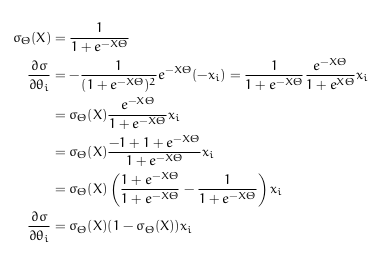
\includegraphics[scale=0.5]{../Figuras/ecuaciones.png}
 %\caption{Gráfica logística.}
 \label{fig:graficaLog}
\end{figure}

Al tener la notación matricial esto me va a permitir más adelante utilizar aquella anotación en la que x tenía hacia abajo todos los ejemplares de entrenamiento que nosotros queramos hacia la derecha todas las dimensiones que necesite para las características de entrada y recordemos también que el vector z lo que tenía era sobre las columnas los pesos correspondientes para calcular las entradas a cada una de las neuronas de salida vamos a decir que tenemos sl neuronas entonces para pensarlo ahorita de manera un poco cómoda me limito al caso de un solo ejemplar este x z sería una versión abreviada de escribir x 0 beta 0 1 pero con ceros unos con unos hasta x n entonces esto es lo que tengo realmente escrito todo es afectado por el signo menos entonces vamos a calcular la derivada de esta función con respecto a cualquiera de estos parámetros y lo vamos a llamar z 
Por la regla de la cadena comenzamos calculando la derivada de 1 entre una función sería menos 1 entre lo que tengo aquí abajo elevado al cuadrado por la derivada de lo de adentro el 1 sería constante entonces no pasa nada me queda solamente ese término derivada del exponencial pues es la misma exponencial derivada de x la derivada de lo que esté en el exponente ahora en el caso del exponente recordemos que es precisamente el menos multiplicando a todo esto que está acá entonces el menos lo vamos a sacar aquí y como la parcial le estoy sacando con respecto a uno de los de los pesos lo único que va a sobrevivir de la derivada de este exponente va a ser precisamente la equis que esté acompañando a la teta con respecto a la cual estoy derivando entonces por eso tenemos aquí la presencia de este xy solito ya que hicimos esto el resto va a ser utilizar un poco de trucos algebraicos para escribirlo de una manera que nos resulte mucho más cómoda realmente el cálculo de la derivada ya lo terminamos hasta aquí vamos a ver ahora qué propiedad descubrimos si tratamos de reescribir esto bueno en primer lugar vamos a cancelar este menos con este menos vayan dando los cargando los dio más este que este que vamos a separar ahorita el dividendo de manera que quede uno entre este elemento la vamos a subir encima del otro observemos que como se están multiplicando pues realmente no hemos hecho nada sólo fue una reescritura y la equis y la vamos a tener ahorita acompañándonos de adorno todo el tiempo así que así recuerden que está aquí en la derecha y ya no nos tenemos que volver a preocupar de ella de ahí en fuera entonces qué vamos a hacer ahora con estos dos elementos lo siguiente es darnos cuenta de que lo que escribimos intencionalmente aquí pues es exactamente sigma ah qué bonito entonces la derivada de esto es lo mismo por otro término que está acá pero resulta que de este término también podemos decir algo interesante el truco favorito de los profesores de cálculo vamos a sumar y restar 1 lo cual es un 0 entonces realmente no modificado nada y otra vez vamos a separar convenientemente cada uno de los términos en particular vamos a observar otra vez este patrón no se hace conocido a la pista vamos a poner este término del lado derecho y uno con  este les va a quedar menos sigma otra vez y los otros dos pues lo ponemos aquí pero a que estamos viendo son idénticos perfecto. Entonces ya tenemos signo esto es realmente dan uno, que siguen otra vez pero con signo negativo entonces lo que tenemos es una propiedad bastante interesante de la función logística. Se está calculando la derivada de sigma con respecto al exponente osea que sería:
Entonces lo que vemos es que la derivada de la sigmoide es la sigmoide por 1 - la sigmoide en este caso bueno como nos interesa en los pesos por eso tenemos aquí un nivel más en la regla de la cadena y nos va a parecer este x,y  en la forma más general vamos a ver que obtener la derivada del gradiente completo se nos va a facilitar mucho entonces vamos a pasar después a la derivada de la función de error.

\begin{figure}[h]
 \centering
 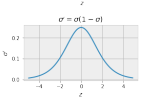
\includegraphics[scale=0.8]{../Figuras/logistica.png}
 \caption{Gráfica logística.}
 \label{fig:graficaLog}
\end{figure}

Las funciones logísticas se utilizan a menudo en redes neuronales para introducir no linealidad en el modelo o para sujetar señales dentro de un intervalo específico . Un elemento de red neuronal popular calcula una combinación lineal de sus señales de entrada y aplica una función logística limitada como función de activación al resultado; este modelo puede verse como una variante "suavizada" de la neurona umbral clásica .

Las funciones logísticas se utilizan en varios roles en estadística. Por ejemplo, son la función de distribución acumulativa de la familia logística de distribuciones y, un poco simplificadas, se utilizan para modelar la posibilidad que tiene un jugador de ajedrez de vencer a su oponente en el sistema de clasificación 

Estas relaciones dan como resultado implementaciones simplificadas de redes neuronales artificiales con neuronas artificiales . Los médicos advierten que las funciones sigmoidales que son antisimétricas con respecto al origen (por ejemplo, la tangente hiperbólica ) conducen a una convergencia más rápida cuando se entrenan redes con retropropagación.

La función logística es en sí misma la derivada de otra función de activación propuesta, el softplus 
Una opción común para la activación o "aplastamiento" funciones, usadas para el clip para grandes magnitudes para mantener la respuesta de la red neuronal limitada 
